\documentclass[12,a4paper]{article}
\usepackage{classiccomputing}

\newcommand\postertype{lightgray}

\begin{document}

\makecclogo

\author{} % owner of the device, also used as "Author" in PDF export
\title{Telekom PrTel 93i / Elmeg aurora}
\def\subtitle{ISDN Prüftelefon}
\def\introduction{Markteinführung 1993}
\makeheader{35}{40} % title size 35, subtitle size 40

\includeimage {images/prtel93i.png}{0.5}

\makebullets{
    Land: Deutschland \newline
    Hersteller: Elmeg im Auftrag der Deutschen Telekom \newline

    Prüftelefon für Installateure der Deutschen Telekom \newline

    Zur Verwendung Am Basisanschluss: \newline
    Mehrgeräteanschluss \newline
    Anlagenanschluss \newline

    Verbindung wahlweise über: \newline
    S0-Schnittstelle (4-draht), oder \newline
    Uk0-Schnittstelle (2-draht) \newline
}

\makemain{
    Protokoll: 1TR6 und ETSI-Euro-ISDN (DSS1) \newline
    \\
    Bitfehlertest (BERT-Test) \newline
    Digitale Schleife (Loopback) \newline
    Auswahl der gesendeten Dienstekennung \newline
    Anklopfen, Rückfrage, Dreierkonferenz, Anrufweiterschaltung \newline
}

%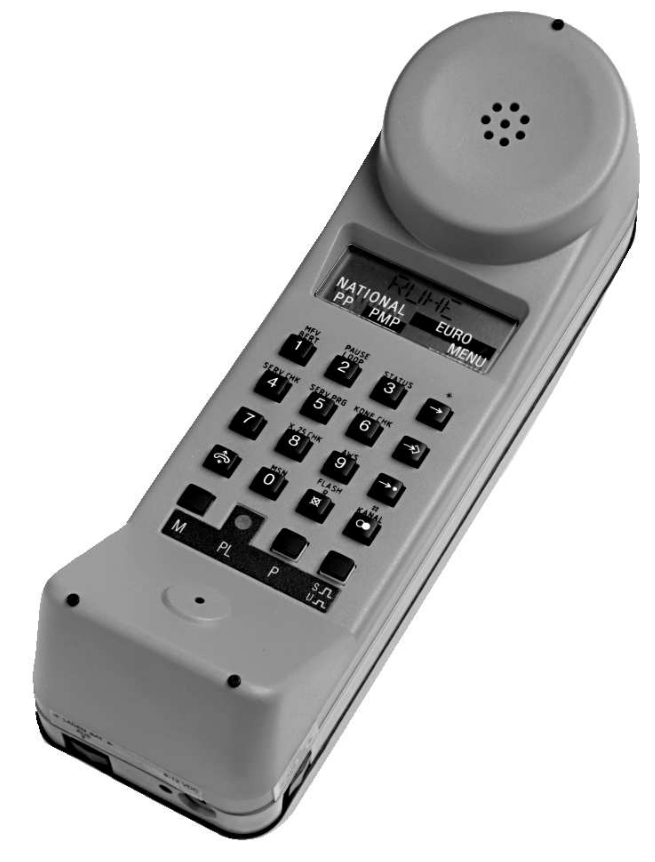
\includegraphics[width=0.5\linewidth]{images/prtel93i.png}

\makefooter

\end{document}
